% =============================================================================
%
% This is the LaTeX source code of the lecture notes.
%
%
% Author:   Blazej Bucha
% Year:     2022
% Contact:  blazej.bucha@stuba.sk
% Encoding: UTF-8
%
% =============================================================================






% LaTeX Packages
% =============================================================================

\documentclass[a4paper, 12pt]{book}
\usepackage[slovak]{babel}
\usepackage[utf8]{inputenc}
\usepackage{listings}
\usepackage{xcolor}
\usepackage[round]{natbib}
\usepackage{graphicx}

% =============================================================================






% Define and set the style of code listings
% =============================================================================

% Define custom colours
\definecolor{comments}{rgb}{0.65, 0.65, 0.65}
\definecolor{strings}{rgb}{0.0, 0.3, 0.6}
\definecolor{linenumbers}{rgb}{0.5, 0.5, 0.5}
\definecolor{keywords}{rgb}{0.85, 0.0, 0.0}
\definecolor{backcolour}{rgb}{0.98, 0.98, 0.98}


% Define custom listing style
\lstdefinestyle{codestyle}
{
    backgroundcolor=\color{backcolour},
    commentstyle=\color{comments},
    keywordstyle=\color{keywords},
    numberstyle=\tiny\color{linenumbers},
    stringstyle=\color{strings},
    basicstyle=\ttfamily\footnotesize,
    breakatwhitespace=false,
    breaklines=true,
    captionpos=b,
    keepspaces=true,
    numbers=left,
    numbersep=5pt,
    showspaces=false,
    showstringspaces=false,
    showtabs=false,
    tabsize=2
}


% Apply the custom listing style
\lstset{style=codestyle}

% =============================================================================






% =============================================================================

\begin{document}






% -----------------------------------------------------------------------------

\chapter*{Úvod}






% -----------------------------------------------------------------------------

\chapter{Fyzikálna geodézia}

\section{Súradnicový systém}

\begin{figure}[bt]
\centering
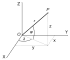
\includegraphics{../figs/coordinate-systems/cart-sph.pdf}
\caption{Pravouhlé a~sférické súradnice v~trojrozmernom pravouhlom súradnicovom 
systéme}
\end{figure}


\section{Polia}

\section{Operátory poľa}

% čo to je?
% súradnicový systém?
% polia
% skalár, vektor, tenzor + ukážky + kódy
% gradient, divergencia, rotácia
% Newtonov gravitačný zákon + pár slov k teórii relativity






% -----------------------------------------------------------------------------

\chapter{Gravitačné a tiažové pole homogénnej gule}

% polia, označenia, jednotky





% -----------------------------------------------------------------------------

\chapter{Gravitačný potenciál všeobecného telesa}

% rozvoj potenciálu do radu sférických harmonických funkcií






% -----------------------------------------------------------------------------

\chapter{Sférické harmonické funkcie}

% čo to je, definícia, porovnanie s jednotkovými vektormi, delenie, ukážka 
% sférických harmonických funkcií v matematickom zápise + obrázky + kód, 
% normovanie, Legendreove polynómy + funkcie, definícia, grafy + kód






% -----------------------------------------------------------------------------

\section{Elipsoidické harmonické funkcie}

% čo to je, definícia, obrázky + grafy + kód, využitie






% -----------------------------------------------------------------------------

\chapter{Normálne tiažové pole}

% čo to je, prečo sa zavádza, ekvipotenciálny elipsoid, základné a odvodené 
% parametre elipsoidu, geometrické a fyzikálne parametre, základné veličiny, 
% stručne opísať normálne pole pomocou elipsoidických harmonických funkcií 
% a vysvetliť výhody takéhoto opisu (uzavreté vzťahy), somiglianov vzťah






% -----------------------------------------------------------------------------

\chapter{Poruchové pole}

% čo to je, prečo sa zavádza, využitie, základné veličiny, vzťahy medzi nimi






% -----------------------------------------------------------------------------

\chapter{Výpočet geoidu}






% -----------------------------------------------------------------------------

\section{Výpočet geoidu rozvojom do radu sférických harmonických funkcií}






% -----------------------------------------------------------------------------

\section{Výpočet geoidu astronomicko--geodetickou niveláciou}






% -----------------------------------------------------------------------------

\section{Výpočet geoidu numerickou integráciou Stokesovho a Hotine integrálov}






% -----------------------------------------------------------------------------

\chapter*{Záver}






% Bibliography
% -----------------------------------------------------------------------------

\bibliographystyle{apalike}
\bibliography{references.bib}

\end{document}

% =============================================================================
% End of the code
